\documentclass[longbibliography,nofootinbib,twocolumn]{revtex4-1}

\newcommand{\network}{The NuCypher Network}

\usepackage{listings}
\usepackage{graphicx}
\usepackage{amsmath}
\usepackage[margin=5pt]{subfig}
\usepackage[usenames]{color}

\renewcommand{\baselinestretch}{1.4}
\setlength{\parskip}{1em}
\definecolor{darkgreen}{rgb}{0.00,0.50,0.25}
\definecolor{darkblue}{rgb}{0.00,0.00,0.67}
\newcommand{\figref}[1]{Fig.~\ref{#1}}
\usepackage[breaklinks,pdftitle={The NuCypher Network: A decentralized
cryptological network offering accessible, intuitive, and extensible runtimes and interfaces for secrets management and dynamic access
control}, pdfauthor={NuCypher},colorlinks,urlcolor=blue,citecolor=darkgreen,linkcolor=darkblue]{hyperref}
\graphicspath{{pdf/}}

\usepackage[T1]{fontenc}
\usepackage{lmodern}
\lstset{
    basicstyle=\ttfamily,
    basewidth={0.5em, 0.5em},
    columns=fullflexible,
}

\begin{document}

\title{\network: A decentralized cryptological network offering accessible, intuitive, and extensible runtimes and interfaces for secrets management and dynamic access control}

\author{Michael Egorov}
\email{michael@nucypher.com}
\author{David Nu{\~n}ez}
\email{david@nucypher.com}
\author{MacLane Wilkison}
\email{maclane@nucypher.com}
\affiliation{NuCypher}

\begin{abstract}
    \network~provides accessible, intuitive, and extensible runtimes and interfaces for secrets management and dynamic access control.
    It's accessible by virtue of being decentralized, permissionless, and censorship-resistant: there are no gate-keepers and anyone can use it.
    It's intuitive thanks to the classic character-based narrative of Alice and Bob (with the introduction of additional cryptological characters
    where appropriate), that permeates the code-base and helps developers write safe, misuse-resistant code.
    It's extensible as it currently supports proxy re-encryption but can be extended to provide support other cryptographic primitives.

    \network~enables developers to manage secrets and dynamically grant and revoke access to sensitive data in public networks.
\end{abstract}

\date{\today}
\maketitle

\tableofcontents

\section{Introduction}

A key management system (KMS) is an integrated approach for generating, distributing, and managing cryptographic keys for devices and
applications~(\figref{fig:kms}).
A KMS includes the backend functionality for key generation, distribution, and rotation as well as the client functionality for
injecting, storing, and managing keys on devices~\cite{wiki:kms}.

\begin{figure}
    \centering
    \subfloat[Centralized KMS]{\includegraphics[width=0.4\columnwidth]{pdf/centralized-kms.pdf}}
    \qquad
    \qquad
    \subfloat[PRE-based KMS]{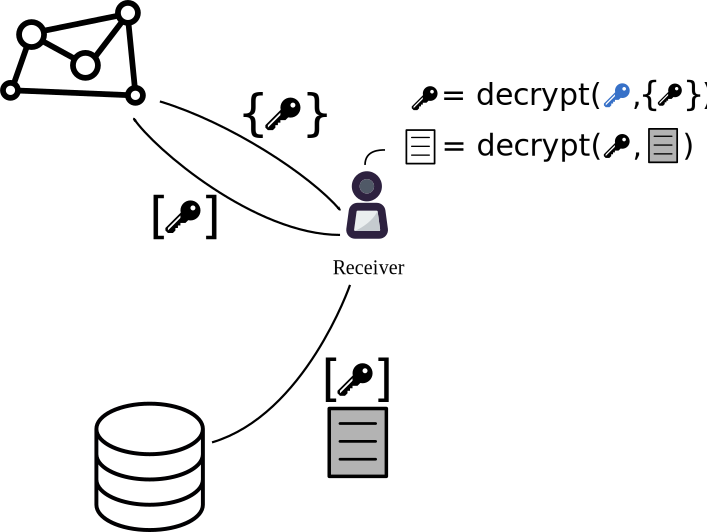
\includegraphics[width=0.4\columnwidth]{pdf/pre-kms.pdf}}
    \caption{Difference between a centralized key management system (KMS) and one which uses proxy re-encryption (PRE)}
    \label{fig:kms}
\end{figure}


As the root of trust, it's critical that a KMS is appropriately configured, managed, and protected.
Historically, this has meant deploying a KMS on-premises in hardware security modules (HSM)~\cite{wiki:hsm} or using tools like
HashiCorp's Vault~\cite{web:hashicorp-vault}.
However, this requires a high degree of technical sophistication as well as upfront capital investment.
To ease the technical burden and provide more competitive pricing, vendors like Amazon CloudHSM~\cite{web:aws-cloudhsm},
Google Cloud KMS~\cite{web:google-cloud-kms}, Azure Key Vault~\cite{web:azure-key-vault} and TrueVault~\cite{web:truevault}
have begun offering KMS as a service.
However, KMS as a service offerings necessitate placing an undue level of trust in the service provider, which may
be inappropriate for security-critical applications.

Public consensus networks, such as Bitcoin and Ethereum, are a promising solution to this centralization problem.
But the limitations of public consensus networks in performing cryptographic operations that involve the manipulation of secret
data are well-established~\cite{cryptoeprint:2017:201}. Consensus networks employ a volunteer network of nodes,
which is subject to constant churn and not as reliable as central infrastructure when it comes to availability and
enforcing access management rules.

\network~ uses a decentralized network to remove the reliance on central service providers, proxy re-encryption for cryptographic
access control, and a token incentive mechanism to ensure reliability, availability, and correctness.
Because of the use of proxy re-encryption, an unencrypted symmetric key (which gives the ability to decrypt private data) is never exposed
server-side~(\figref{fig:kms}), and there is no single point of security failure.
Even if compromised, hackers would only get re-encryption keys but access to the file is still protected.

\section{Network}

\section{Smart contract layer}

\section{NU token and staking economics}

\section{Characters}

\section{Conclusion}

\bibliography{whitepaper}

\end{document}
